\subsubsection{16.01.2016}
\textit{\textbf{Time frame:}} 16:00-21:30

There was created a moving mount for one of the ribs at the elevator (figure \ref{Elevator3.4}).

It was also developed a prototype of a mechanism for grasping the hurdle at the ramp. The construction of the transfer between the servo and the hooks will prevent the servo from breaking down (figure \ref{Hooks1.2}).

\begin{figure}[H]
	\begin{minipage}[h]{0.47\linewidth}
		\center{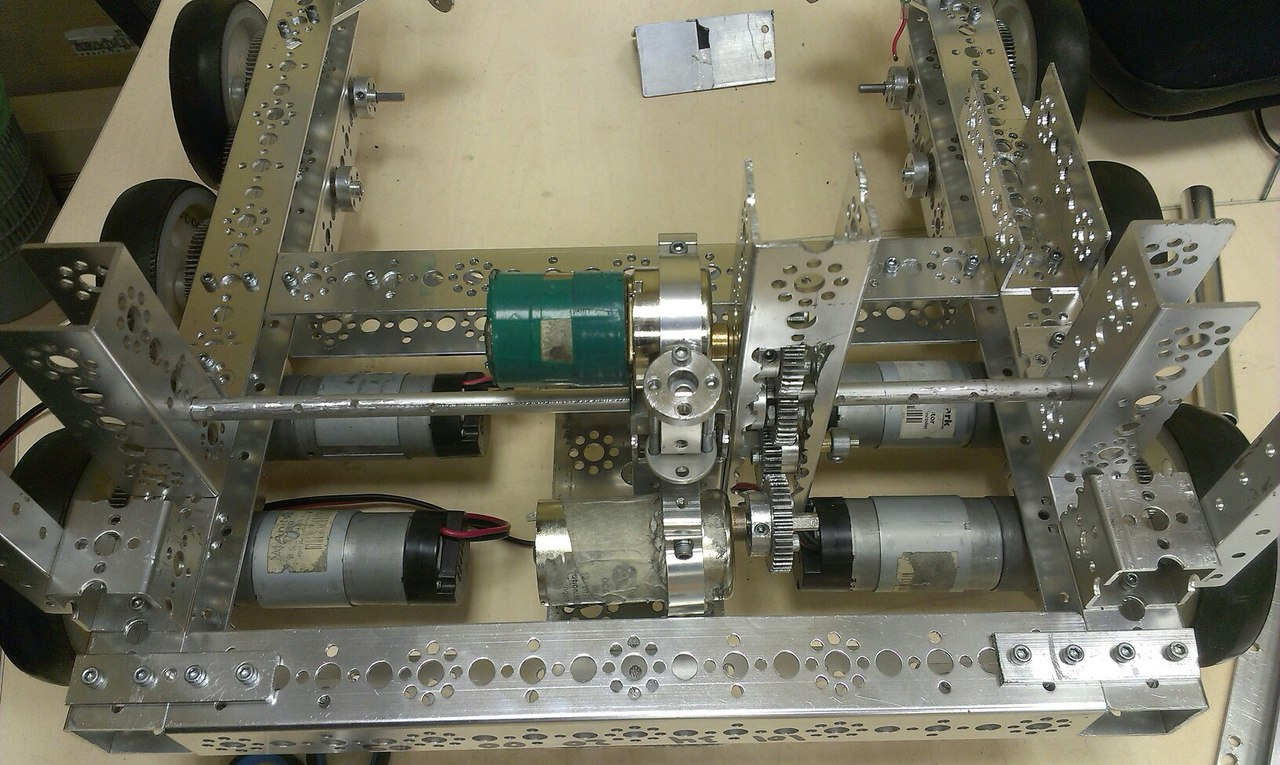
\includegraphics[scale=0.2]{3Engineering/5Team_meetings/days_of_meetings/2016.01.16/images/01}}
		\caption{Moving mount of a rib}
		\label{Elevator3.4}
	\end{minipage}
	\hfill
	\begin{minipage}[h]{0.47\linewidth}
		\center{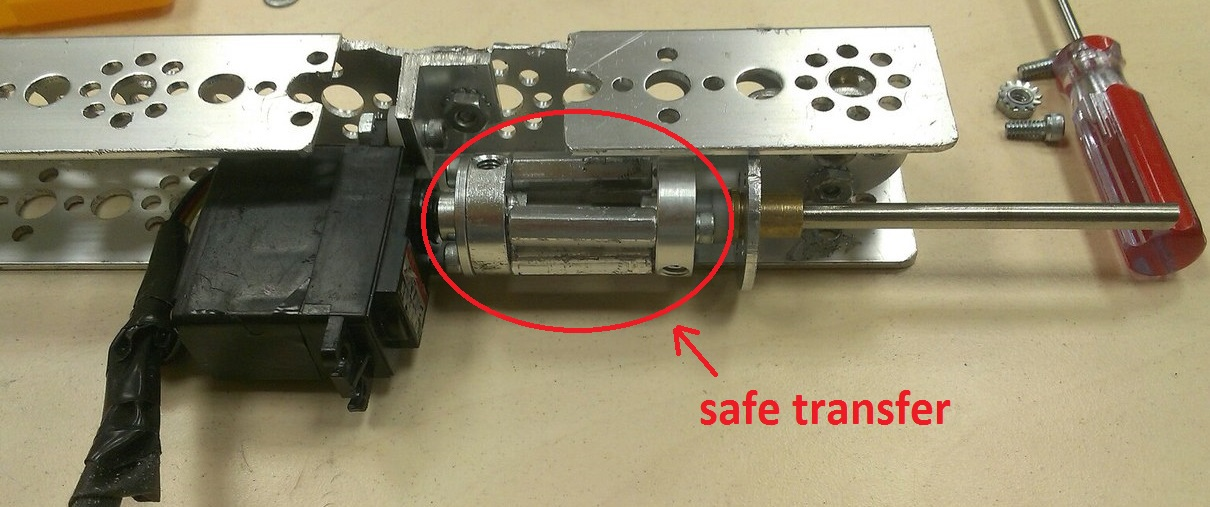
\includegraphics[scale=0.22]{3Engineering/5Team_meetings/days_of_meetings/2016.01.16/images/02}}
		\caption{A prototype of the mechanism for grasping the hurdle}
		\label{Hooks1.2}
	\end{minipage}
\end{figure}
